\documentclass[fleqn,11pt]{article}

\usepackage[letterpaper,margin=0.75in]{geometry}

\usepackage{amsmath}
\usepackage{booktabs}
\usepackage{graphicx}
\usepackage{listings}

\setlength{\parindent}{1.4em}

\begin{document}

\lstset{
  language=Python,
  basicstyle=\small,          % print whole listing small
  keywordstyle=\bfseries,
  identifierstyle=,           % nothing happens
  commentstyle=,              % white comments
  stringstyle=\ttfamily,      % typewriter type for strings
  showstringspaces=false,     % no special string spaces
  numbers=left,
  numberstyle=\tiny,
  numbersep=5pt,
  frame=tb,
}

\title{Congestion Control Part 1 (Lab 3) Report}

\author{Luke Dickinson}

\date{3/18/2017}

\maketitle

\section{Introduction}

Congestion control for TCP allows connections to slow down or speed up depending on current network conditions. While there are a number of congestion control algorithms for TCP, we will look at the effects of congestion control written for TCP Tahoe. TCP Tahoe performs a slow start at any loss detected (a timeout or three duplicate ACKs). At the beginning of slow start, the congestion window size is reduced down to 1 mss and the threshold is cut in half. During slow start, the congestion window size grows for every packet successfully acknowledged. When the congestion window size reaches the threshold, slow start is replaced with additive increase. Additive increase increases the congestion window as well, but at a much slower speed.

\section{Experiments}
The experiments performed include a network that consisting of 2 nodes. We set the bandwidth between the nodes to 1 Mbps and set the propagation delay between the nodes to 100 ms. We will set the initial window size to 1,000 and the threshold value to 100,000. We set our mss to 1,000. We will send the "internet-architecture.pdf" file.

\subsection{No packet loss}
For the first simulation, we use the network described above. There is no packet loss. We record the window size as it changes from TCP Tahoe's congestion control. \\\\
This simulation uses following command: python lab3-basic-1.py -f internet-architecture.pdf -r\\

The congestion window size graph is shown here:

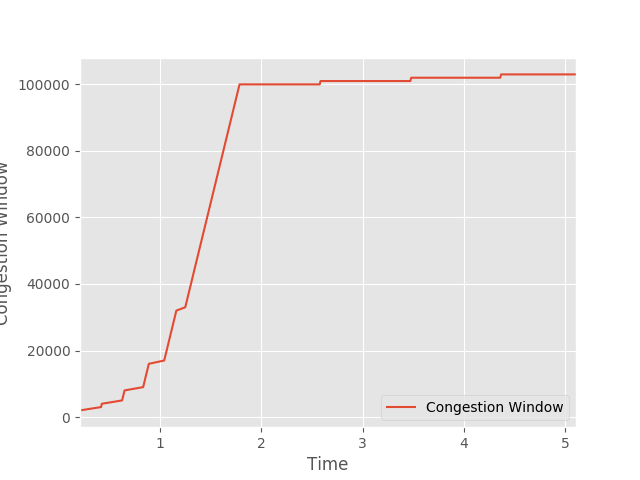
\includegraphics[width=11cm]{cwnd1}\\

 \subsection{1 packet is lost}
For the second simulation, we use the network described above. There is packet loss at sequence number 14,000. We record the window size as it changes from TCP Tahoe's congestion control. We also record the traffic as packets are successfully received, packets are lost, and when ACKs are received. \\\\
This simulation uses the following command: python lab3-basic-2.py -f internet-architecture.pdf -r\\ 

The congestion window size graph is shown here:

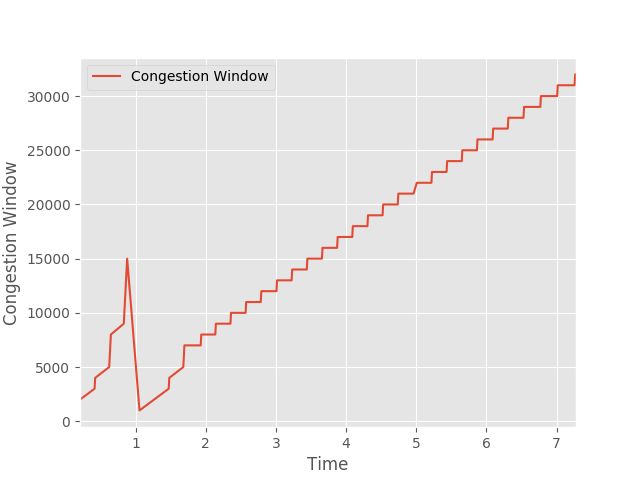
\includegraphics[width=11cm]{cwnd2}\\

The packet traffic graph is shown here:

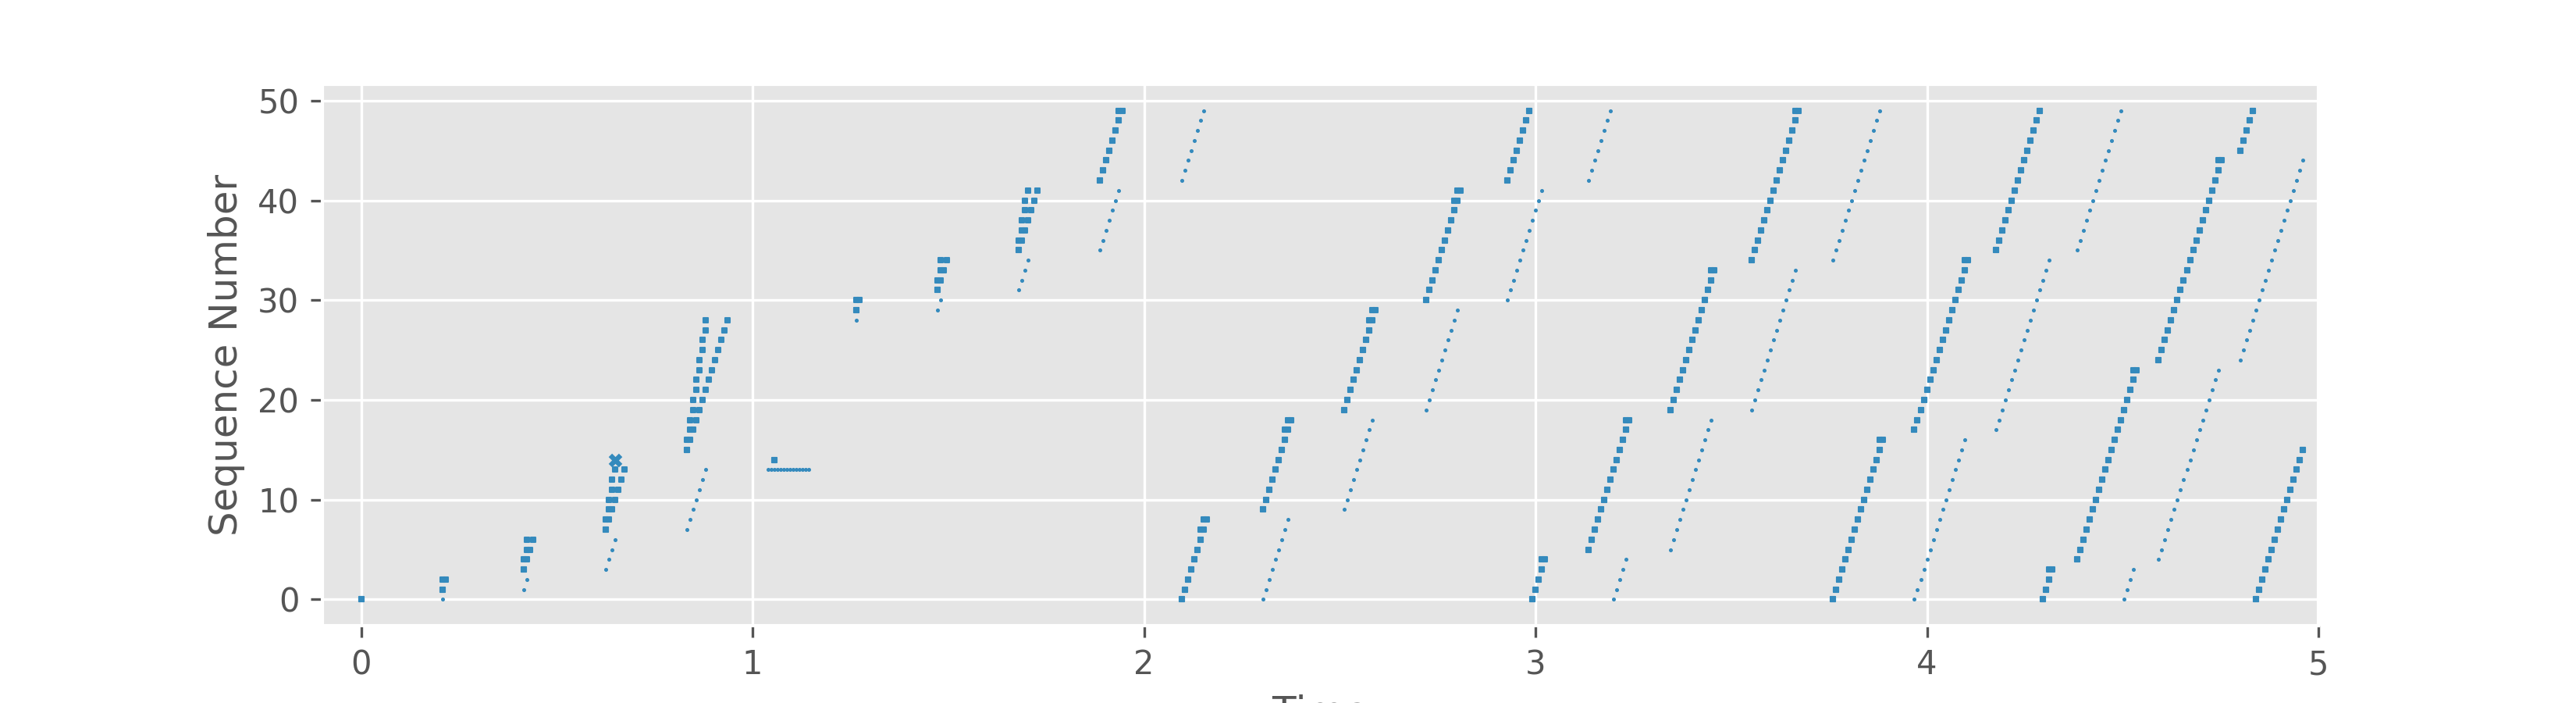
\includegraphics[width=11cm]{sequence2}\\

\subsection{2 packets are lost}
For the third simulation, we use the network described above. There is packet loss at sequence numbers 14,000 and 28,000. We record the window size as it changes from TCP Tahoe's congestion control. We also record the traffic as packets are successfully received, packets are lost, and when ACKs are received.\\\\
This simulation uses the following command: python lab3-basic-3.py -f internet-architecture.pdf -r\\

The congestion window size graph is shown here:

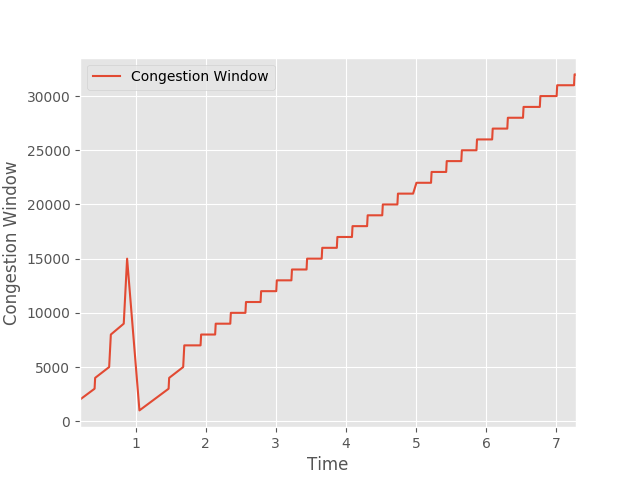
\includegraphics[width=11cm]{cwnd3}\\

The packet traffic graph is shown here:

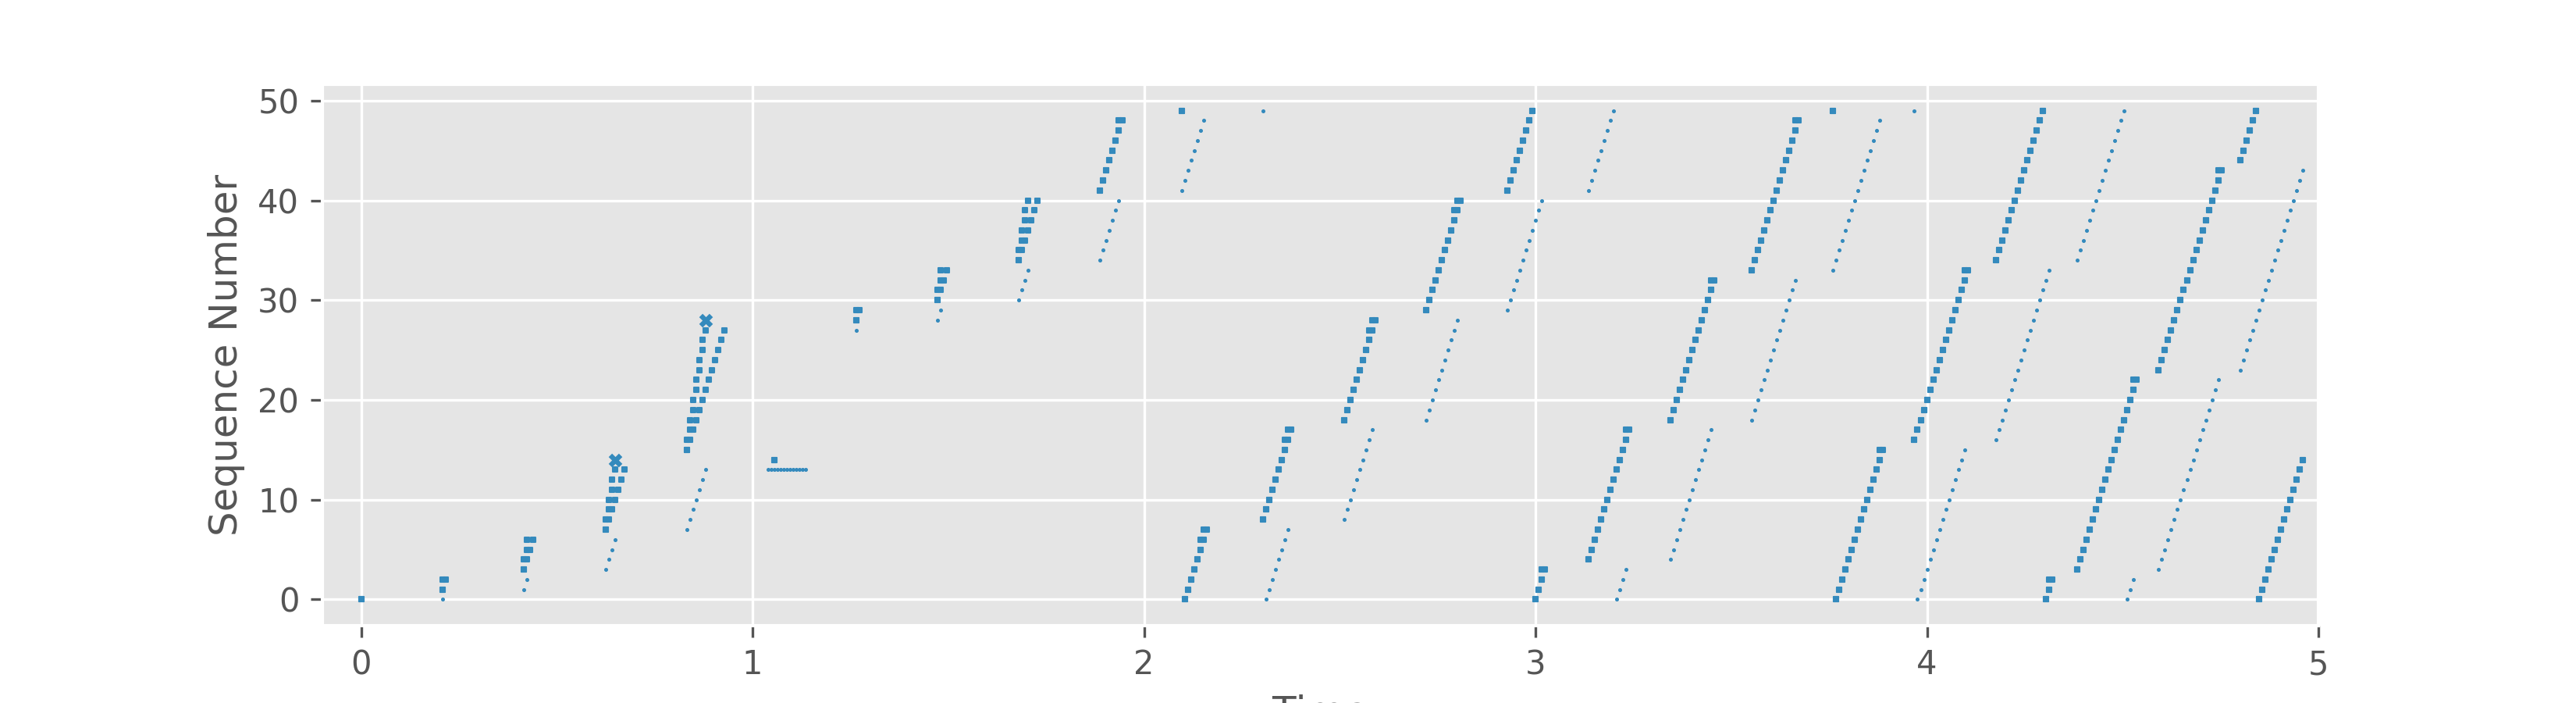
\includegraphics[width=11cm]{sequence3}\\

\subsection{3 packets are lost}
For the fourth simulation, we use the network described above. There is packet loss at sequence numbers 14,000, 26,000, and 28,000. We record the window size as it changes from TCP Tahoe's congestion control. We also record the traffic as packets are successfully received, packets are lost, and when ACKs are received.\\\\
This simulation uses the following command: python lab3-basic-4.py -f internet-architecture.pdf -r\\

The congestion window size graph is shown here:

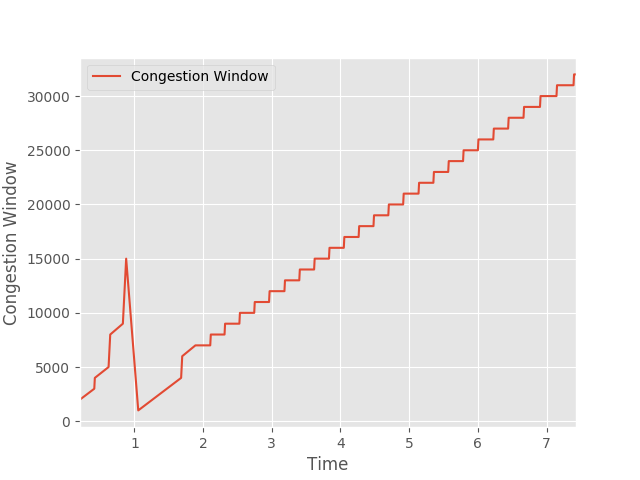
\includegraphics[width=11cm]{cwnd4}\\

The packet traffic graph is shown here:

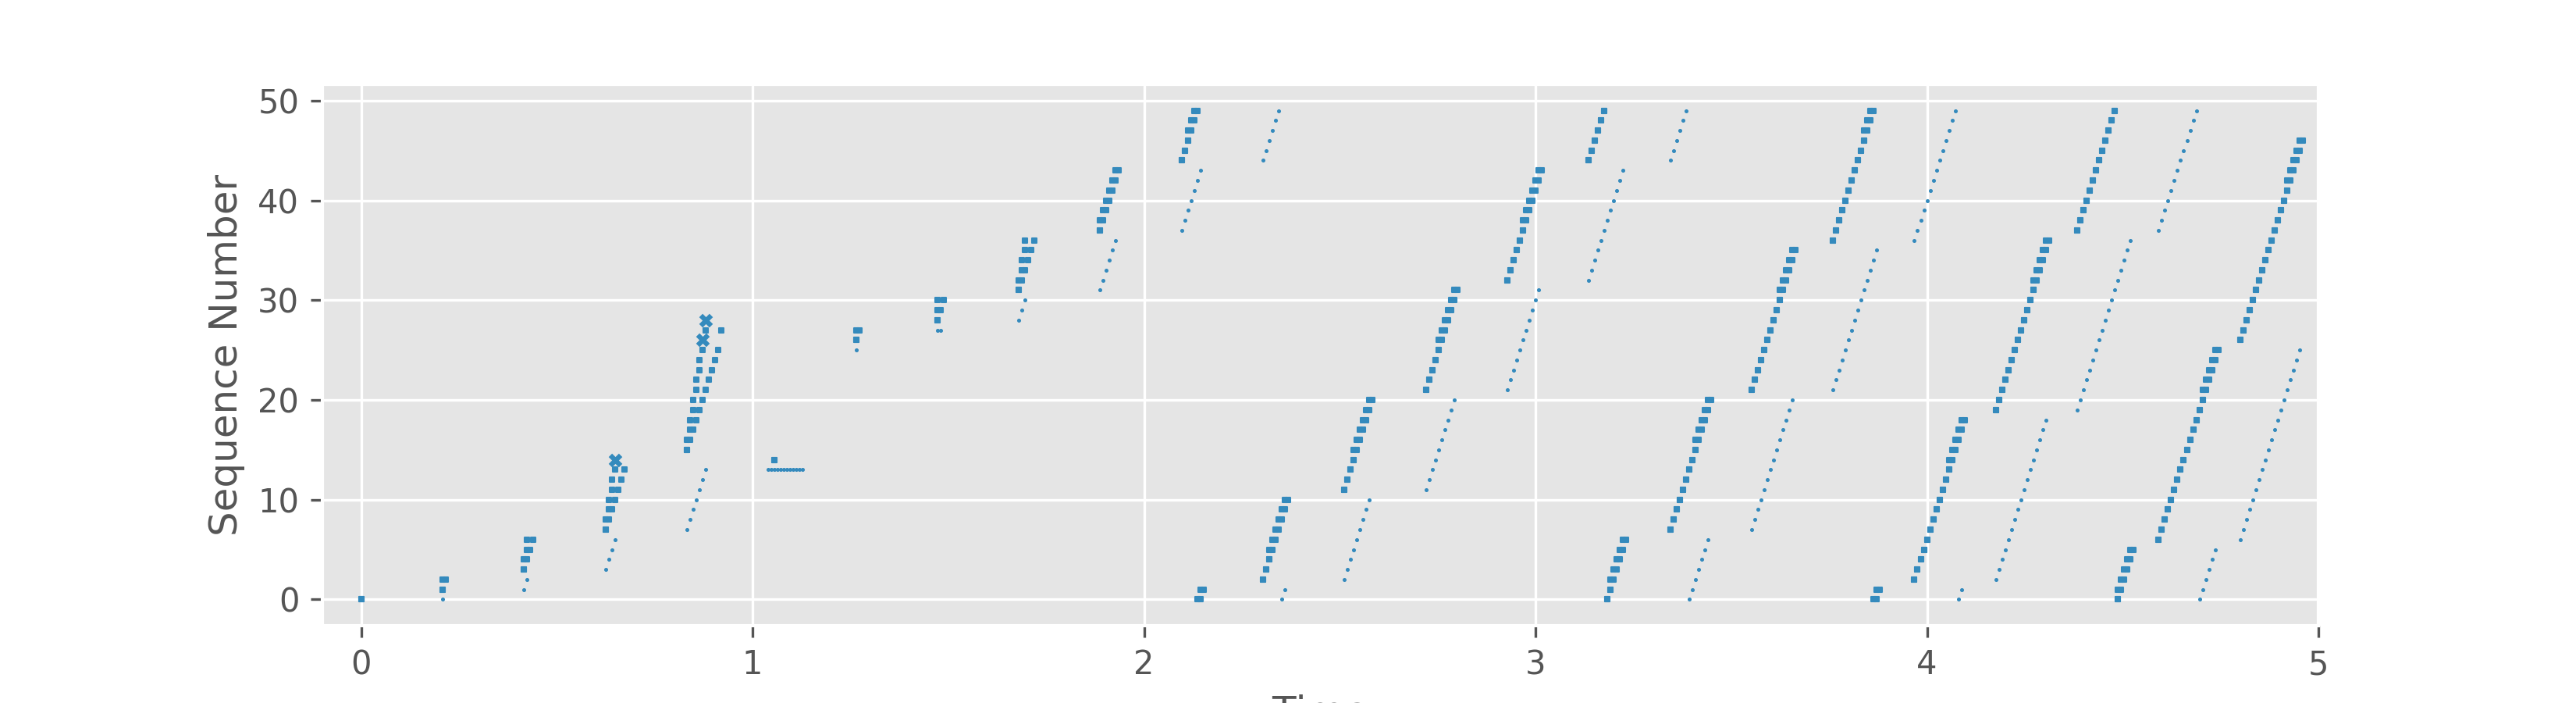
\includegraphics[width=11cm]{sequence4}\\

\section{Discussion}
The data from our packet traffic graphs and the graphs in the SACK paper are the same. The only difference between the two is the sequence number mod, as the SACK paper used 60 and we used 50.

When comparing the congestion window graph from dropping a single packet and from dropping two packets, we find they are exactly the same. This is because in the situation where two packets were dropped, the second packet was resent after the first dropped packet received an ACK. Basically, the loss from the second packet was completely covered up by the effect of the loss from the first packet.

When comparing the situation where three packets are lost, there is a noticeable change to the congestion window graph. This is because the second packet was resent before the first dropped packet received an ACK, resulting in a new detected loss event.


\end{document}
